\documentclass[hyperref]{beamer}
\usepackage{beamerthemesplit}
\usepackage{graphicx}
\usepackage{mathptmx}           % replacement for obsolete \usepackage{times}
\usepackage[scaled=1.0]{helvet} % replacement for obsolete \usepackage{times}
\usepackage{courier}            % replacement for obsolete \usepackage{times}
\usepackage[normalem]{ulem}

\usepackage{tikz}
\usetikzlibrary{shapes.arrows,chains,positioning,automata,trees,calc}
\usetikzlibrary{patterns}
\usetikzlibrary{decorations.pathmorphing,decorations.markings}
\usepackage{times,latexsym,amsfonts,amssymb,amsmath,graphicx,url,bbm,rotating,siunitx}
\usepackage{multirow,hhline,arydshln,array,color,stmaryrd,pifont,transparent}
\usepackage[absolute,overlay]{textpos}
\definecolor{darkred}{rgb}{0.5, 0.0, 0.0}
\definecolor{darkgreen}{rgb}{0.0, 0.4, 0.0}
\definecolor{darkblue}{rgb}{0.0, 0.0, 0.5}

% set up Beamer style with Stanford colors and logo
% logo is available at http://nlp.stanford.edu/local/nlp-logos/nlp-logo.pdf
\useinnertheme{rounded}
\useoutertheme{infolines}
\usecolortheme{beaver}
\setbeamercolor{block title}{fg=white,bg=darkred!75!black}
\setbeamercolor{block body}{parent=normal text,bg=black!5!bg}
\setbeamercolor{item projected}{bg=darkred}
\logo{
\includegraphics[height=1cm]{nlp-logo.pdf}}

% Macros
\def\blue#1{\textcolor{blue}{#1}}
\def\darkblue#1{\textcolor{blue}{#1}}
\def\red#1{\textcolor{red}{#1}}
\def\darkred#1{\textcolor{darkred}{#1}}
\def\green#1{\textcolor{green}{#1}}
\def\darkgreen#1{\textcolor{darkgreen}{#1}}
\def\yellow#1{\textcolor{yellow}{#1}}
\def\orange#1{\textcolor{orange}{#1}}
\def\gray#1{\textcolor{gray}{#1}}
\def\darkgray#1{\textcolor{darkgray}{#1}}
\newcommand\w[1]{\textit{\darkgreen{#1}}}
\newcommand\ww[1]{\textit{#1}}
\newcommand\h[1]{\textbf{#1}}
\newcommand\hh[1]{\textbf{\textcolor[rgb]{0.5,0,0}{#1}}}

\input ../std-macros.tex

% title page information
\title[Robust Subgraphs for AMR]{Robust Subgraph Generation for Abstract Meaning Representation
Parsing}
\subtitle{}
\author[Werling, Angeli, Manning]{Keenon Werling, \darkblue{Gabor Angeli}, Chris Manning}
\date{May 30, 2015}
\institute[Stanford]{Stanford University}


\begin{document}
\begin{frame}[noframenumbering]
  \titlepage
\end{frame}

%%%%%%%%%%%%%%%%%%%%%%%%%%%%%%%%%%%%%%%%%%%%%%%%%%%%%%%%%%%%%%%%%%%%%%%%%%%%%%%
% What is AMR?
%%%%%%%%%%%%%%%%%%%%%%%%%%%%%%%%%%%%%%%%%%%%%%%%%%%%%%%%%%%%%%%%%%%%%%%%%%%%%%%

\begin{frame}[noframenumbering]{Keenon Werling}
\begin{center}
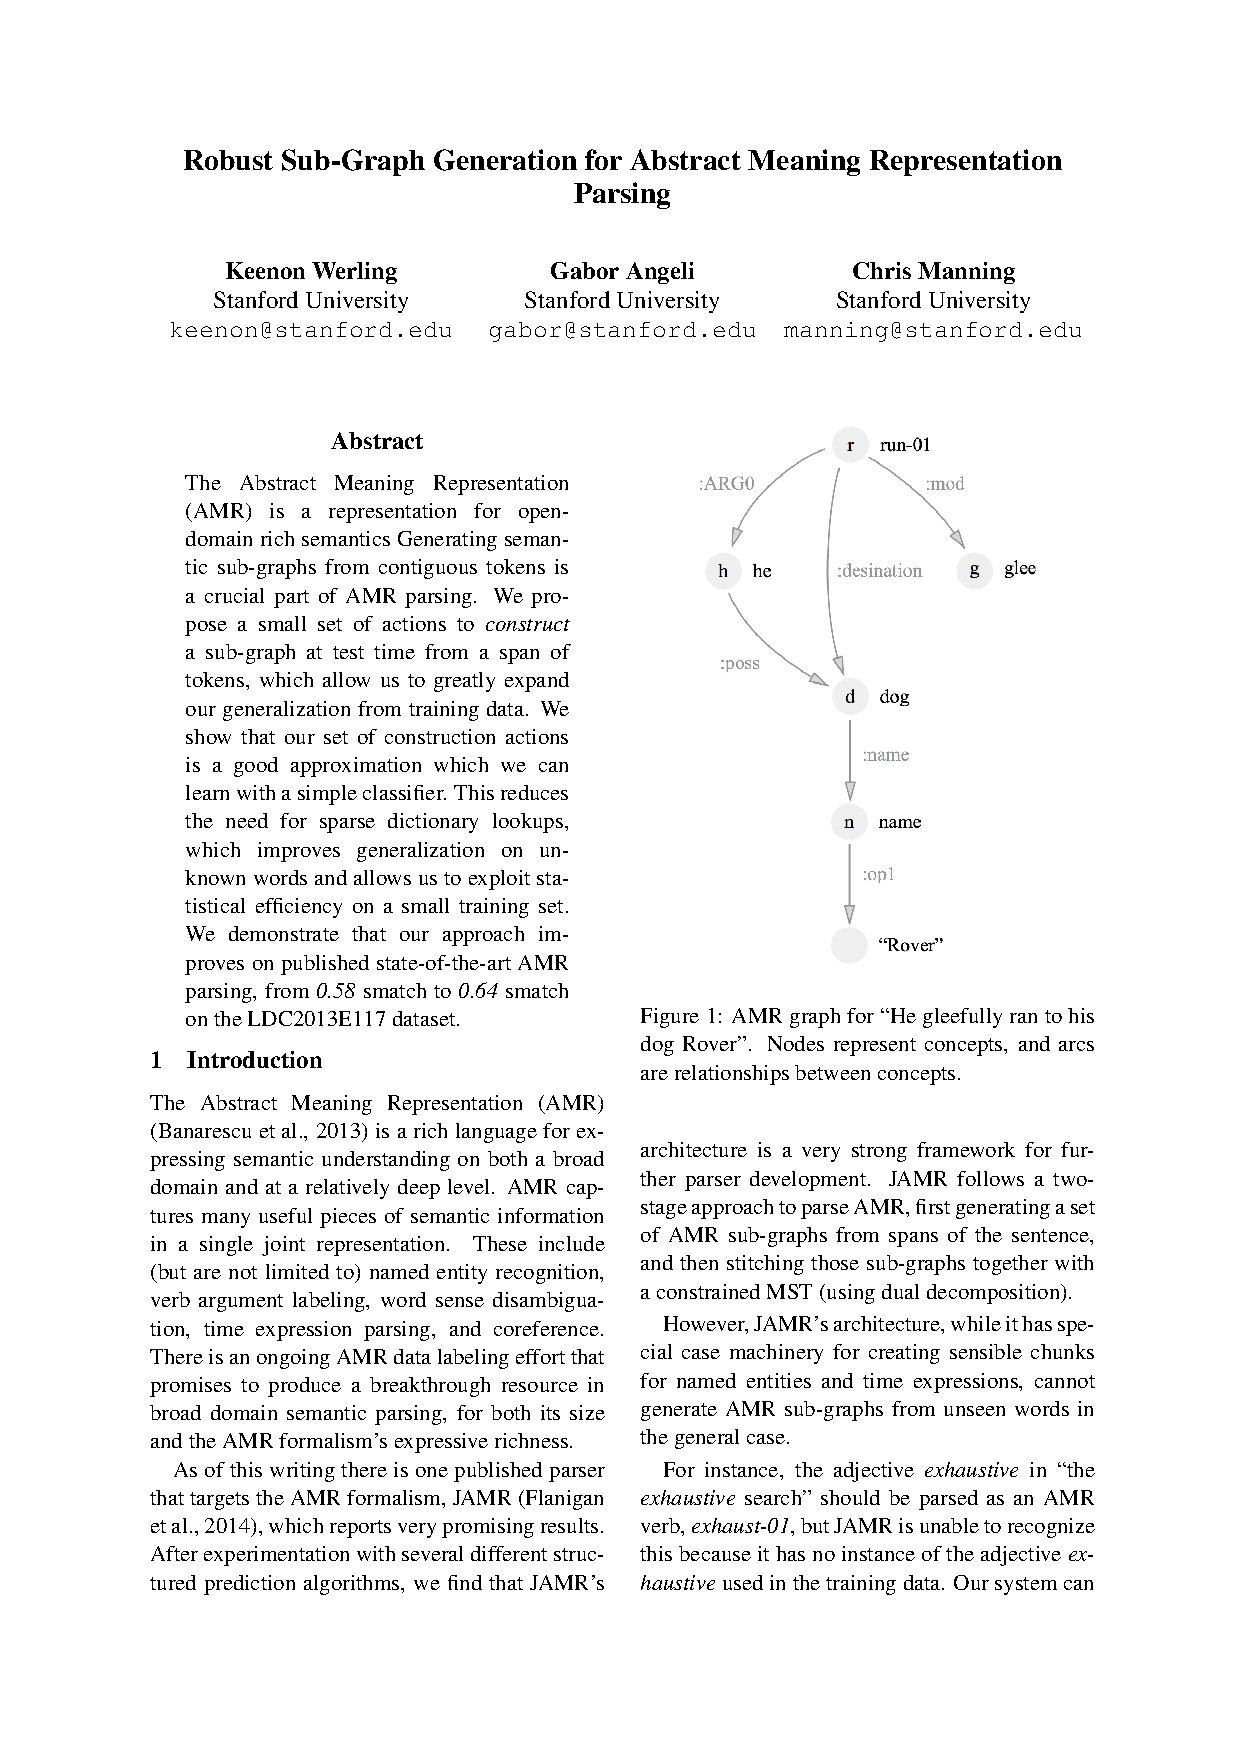
\includegraphics[scale=0.15]{keenon.jpg}
\newline
TODO A picture of Keenon
\end{center}
\end{frame}

%%%%%%%%%%%%%%%%%%% 
% Intro
%%%%%%%%%%%%%%%%%%%
\begin{frame}{What is The Abstract Meaning Representation?}
\begin{center}
\hh{A semantic representation for language as a rooted, directed graph}
\end{center}
\begin{tabular}{lcl}
\w{``He gleefully ran to his dog rover''} &
$\rightarrow$ &
\raisebox{-.5\height}{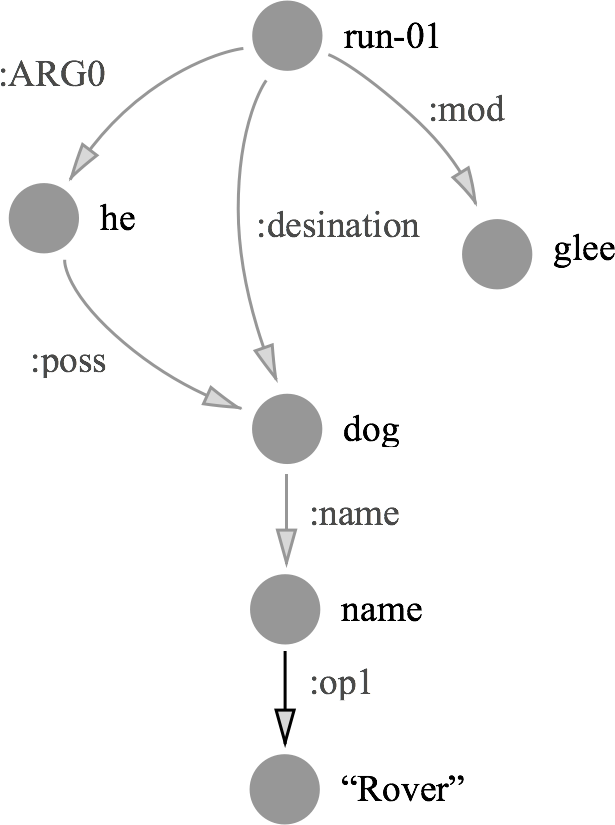
\includegraphics[scale=0.20]{glee.png}}
\end{tabular}
\end{frame}

%%%%%%%%%%%%%%%%%%% 
% Decompose AMR
%%%%%%%%%%%%%%%%%%%
\begin{frame}{Decomposing AMR}
\begin{center}
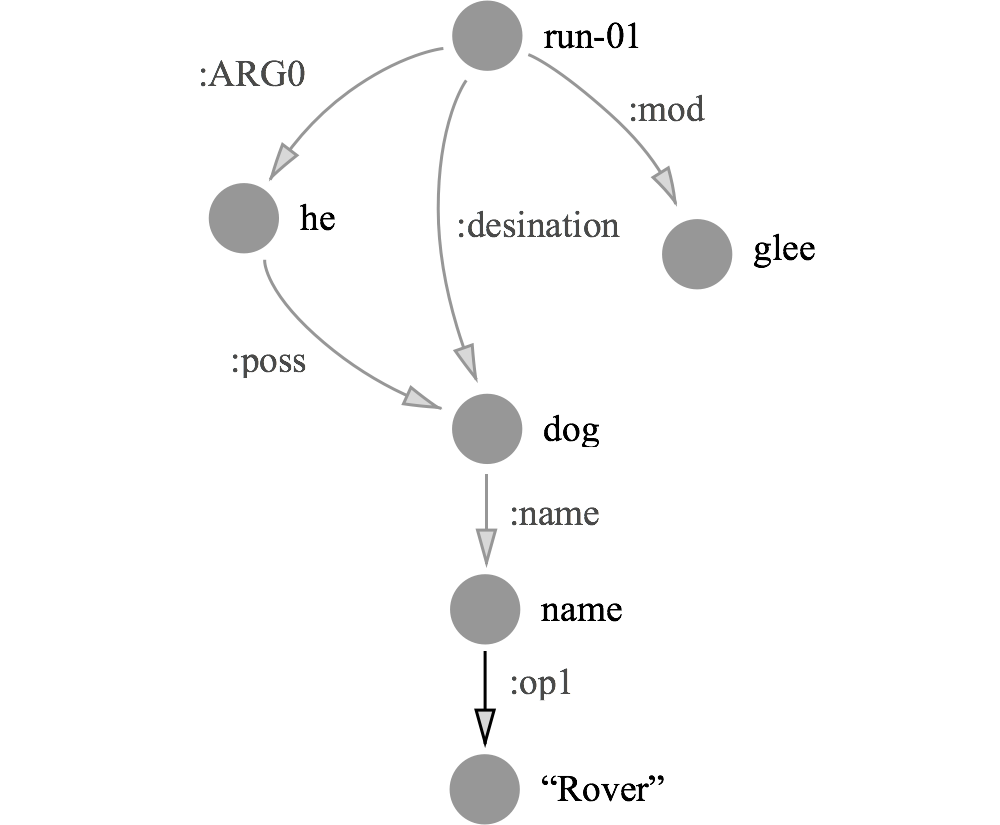
\includegraphics[scale=0.25]{glee_base.png}
\end{center}
\end{frame}

\begin{frame}[noframenumbering]{Decomposing AMR}
\begin{center}
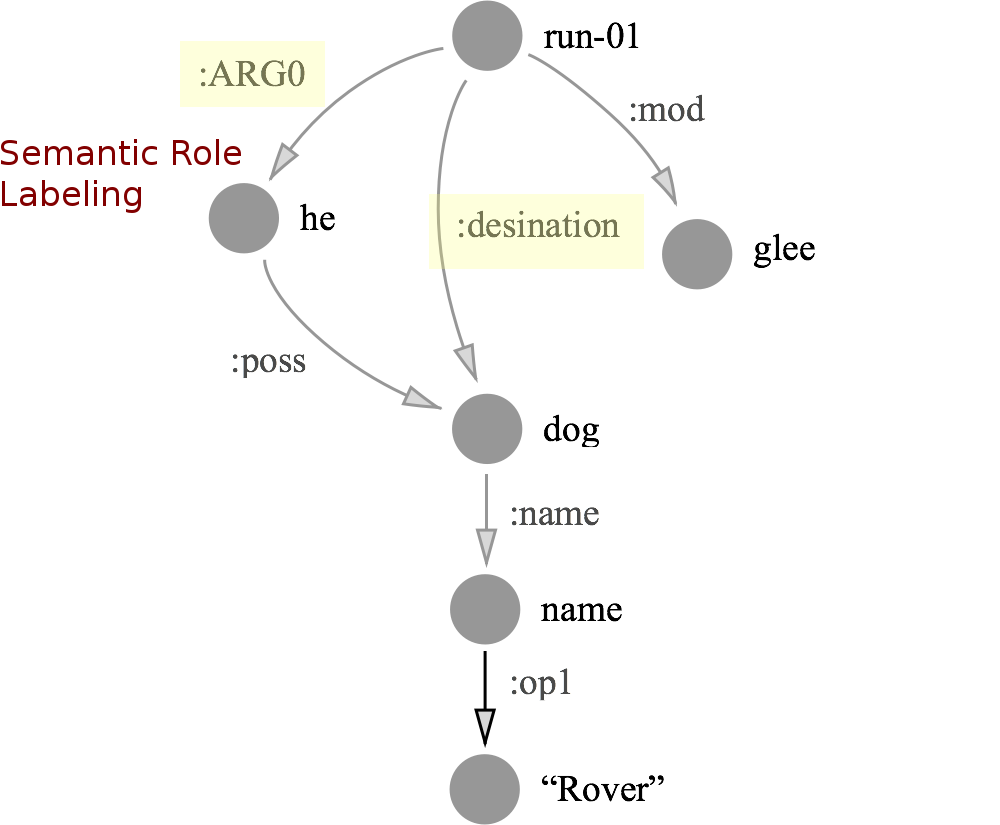
\includegraphics[scale=0.25]{glee_srl.png}
\end{center}
\end{frame}

\begin{frame}[noframenumbering]{Decomposing AMR}
\begin{center}
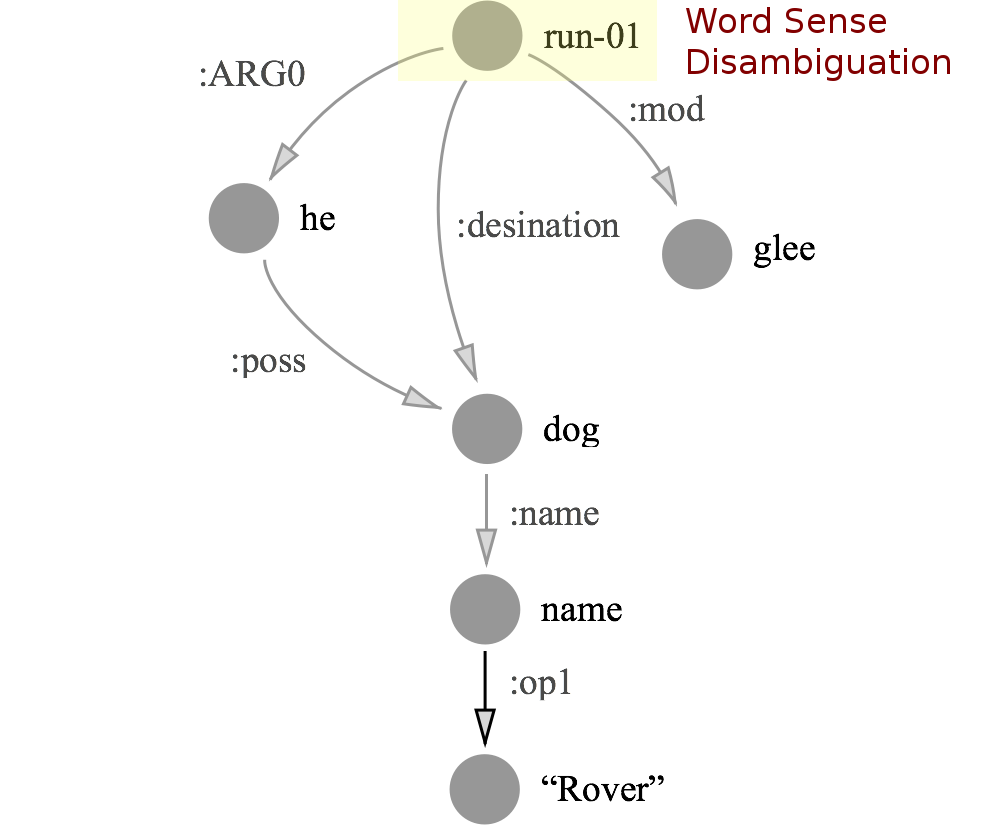
\includegraphics[scale=0.25]{glee_wsd.png}
\end{center}
\end{frame}

\begin{frame}[noframenumbering]{Decomposing AMR}
\begin{center}
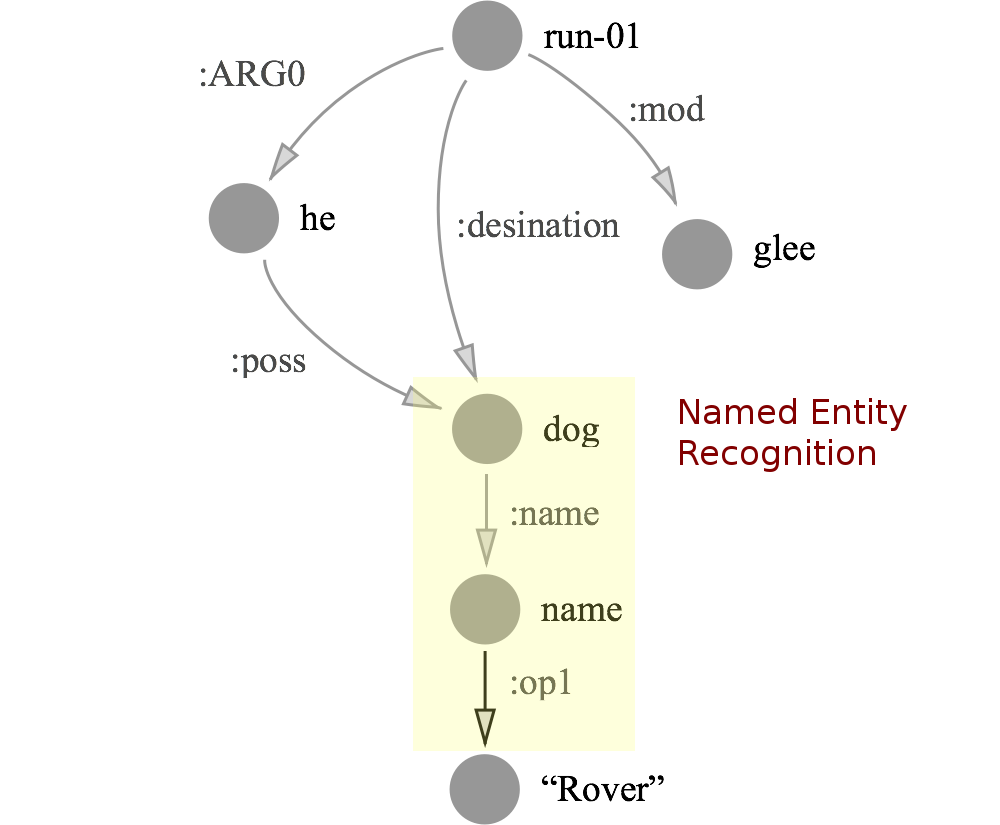
\includegraphics[scale=0.25]{glee_ner.png}
\end{center}
\end{frame}

\begin{frame}[noframenumbering]{Decomposing AMR}
\begin{center}
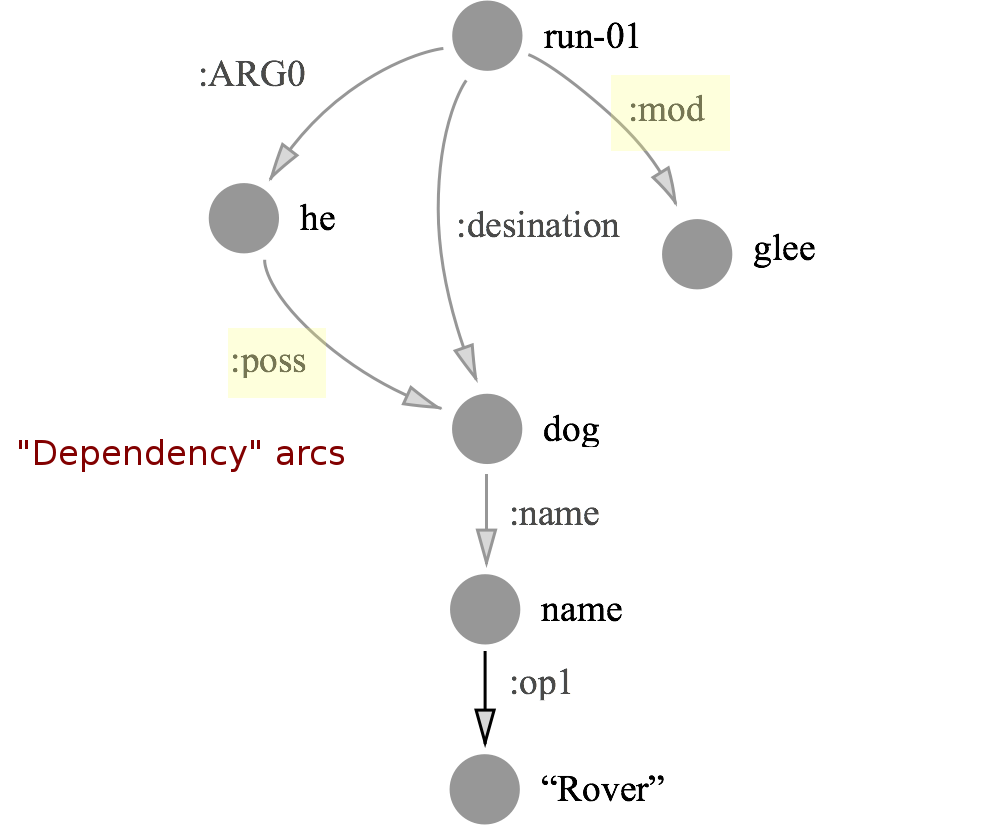
\includegraphics[scale=0.25]{glee_deps.png}
\end{center}
\end{frame}

%%%%%%%%%%%%%%%%%%% 
% NER++ and SRL++
%%%%%%%%%%%%%%%%%%%
\begin{frame}{Insight from JAMR: Two Classes of Phenomena}
\begin{center}
\begin{tabular}{cc}
``SRL++''& \raisebox{-0.5\height}{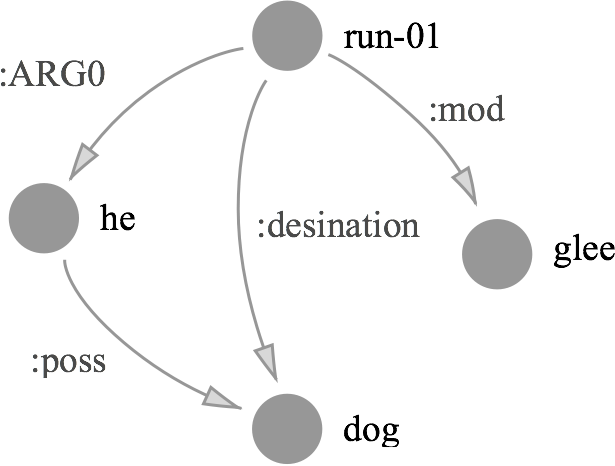
\includegraphics[scale=0.20]{srl_only.png}} \\
& \\
``NER++'' & \raisebox{-0.5\height}{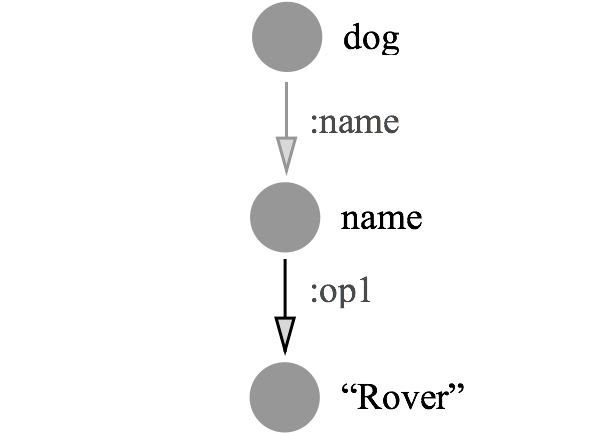
\includegraphics[scale=0.20]{ner_only.png}} \\
\end{tabular}
\end{center}
\end{frame}


%%%%%%%%%%%%%%%%%%% 
% Pipeline
%%%%%%%%%%%%%%%%%%%
\begin{frame}{Pipeline: Start with text}
\begin{center}
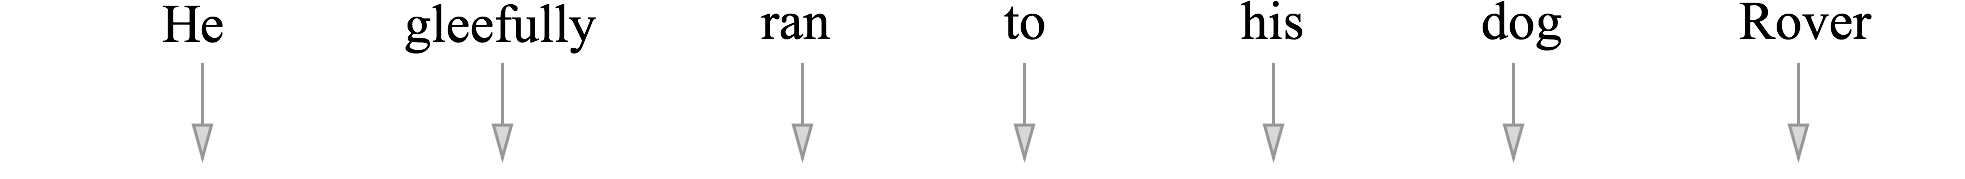
\includegraphics[scale=0.17]{concept_1.png}
\end{center}
\end{frame}

\begin{frame}[noframenumbering]{Pipeline: Generate subgraphs}
\begin{center}
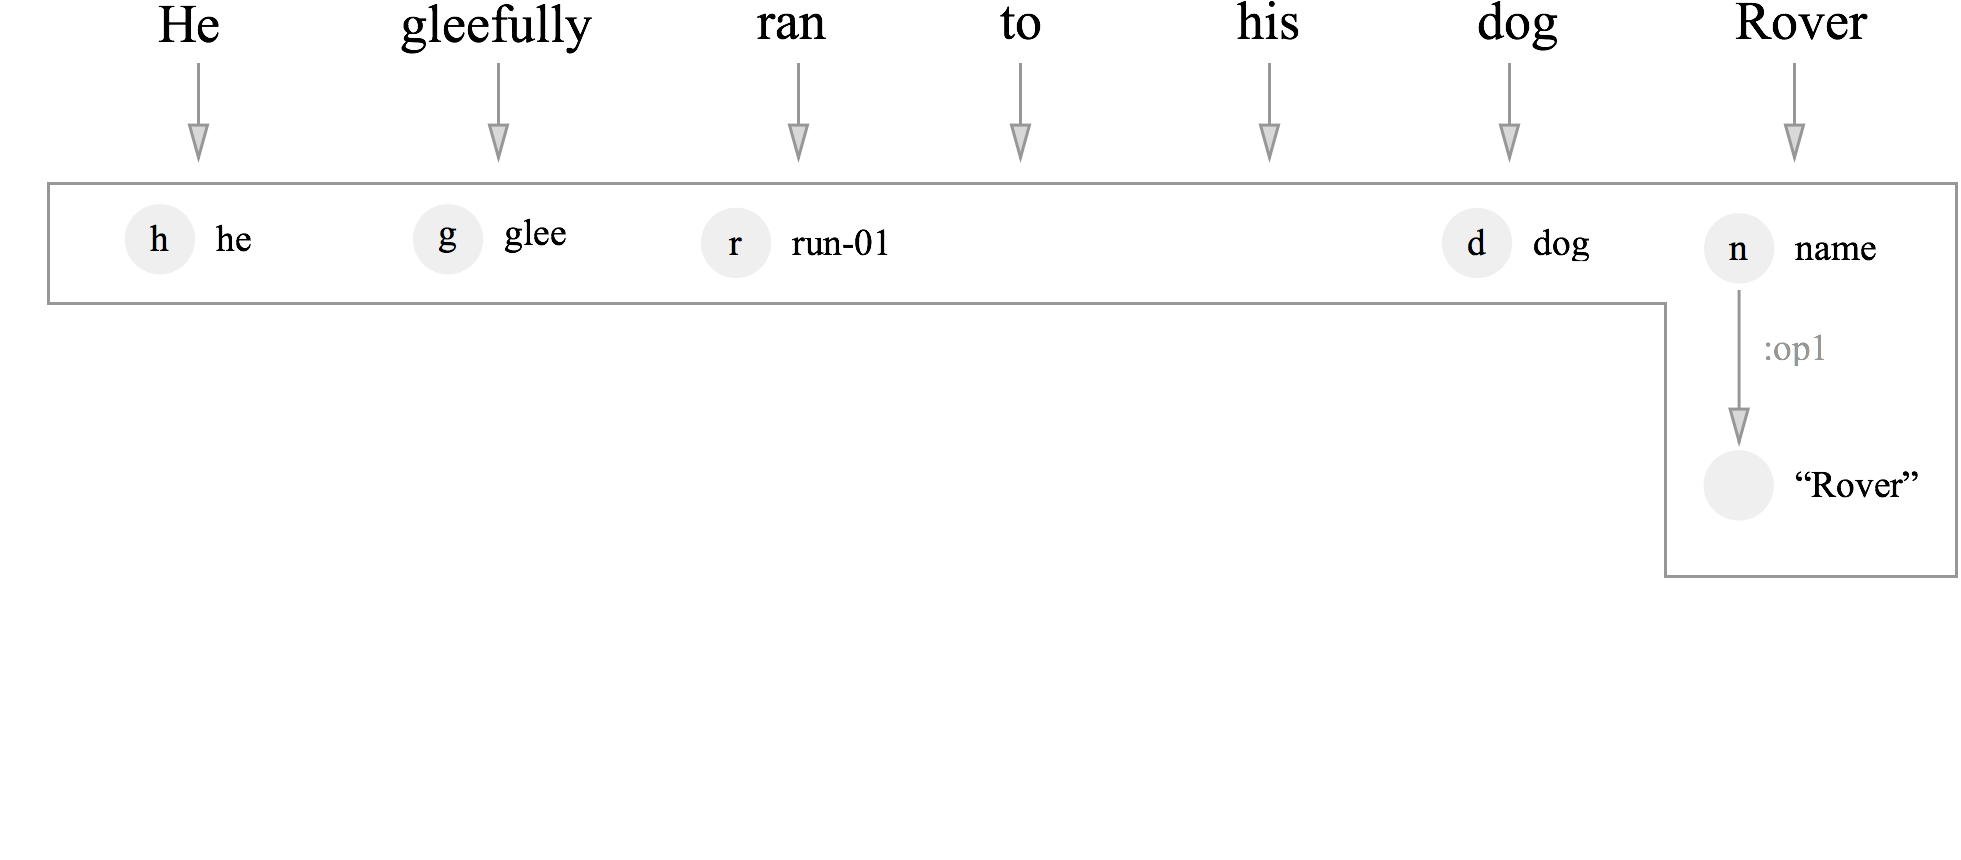
\includegraphics[scale=0.17]{concept_2.png}
\end{center}
\end{frame}

\begin{frame}[noframenumbering]{Pipeline: Link subgraphs}
\begin{center}
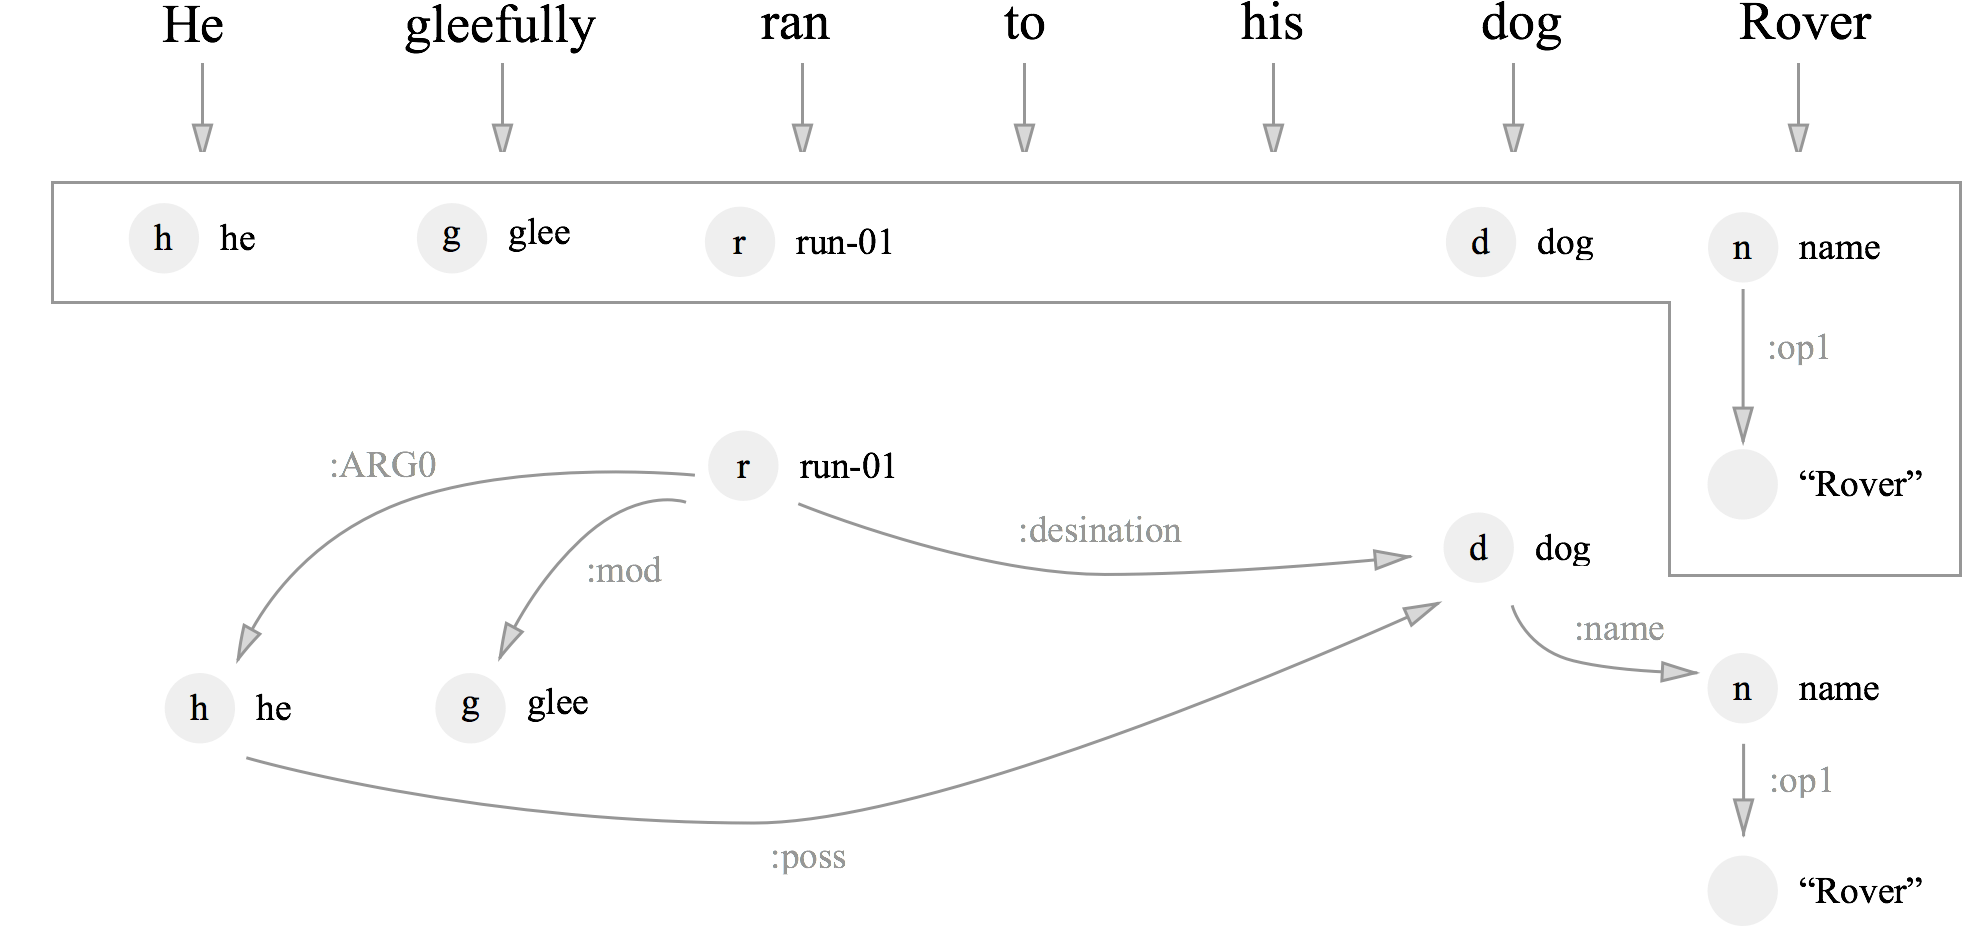
\includegraphics[scale=0.17]{concept_3.png}
\end{center}
\end{frame}


%%%%%%%%%%%%%%%%%%% 
% NER++ is hard
%%%%%%%%%%%%%%%%%%%
\begin{frame}{Observation: NER++ is Surprisingly Hard}
\begin{center}
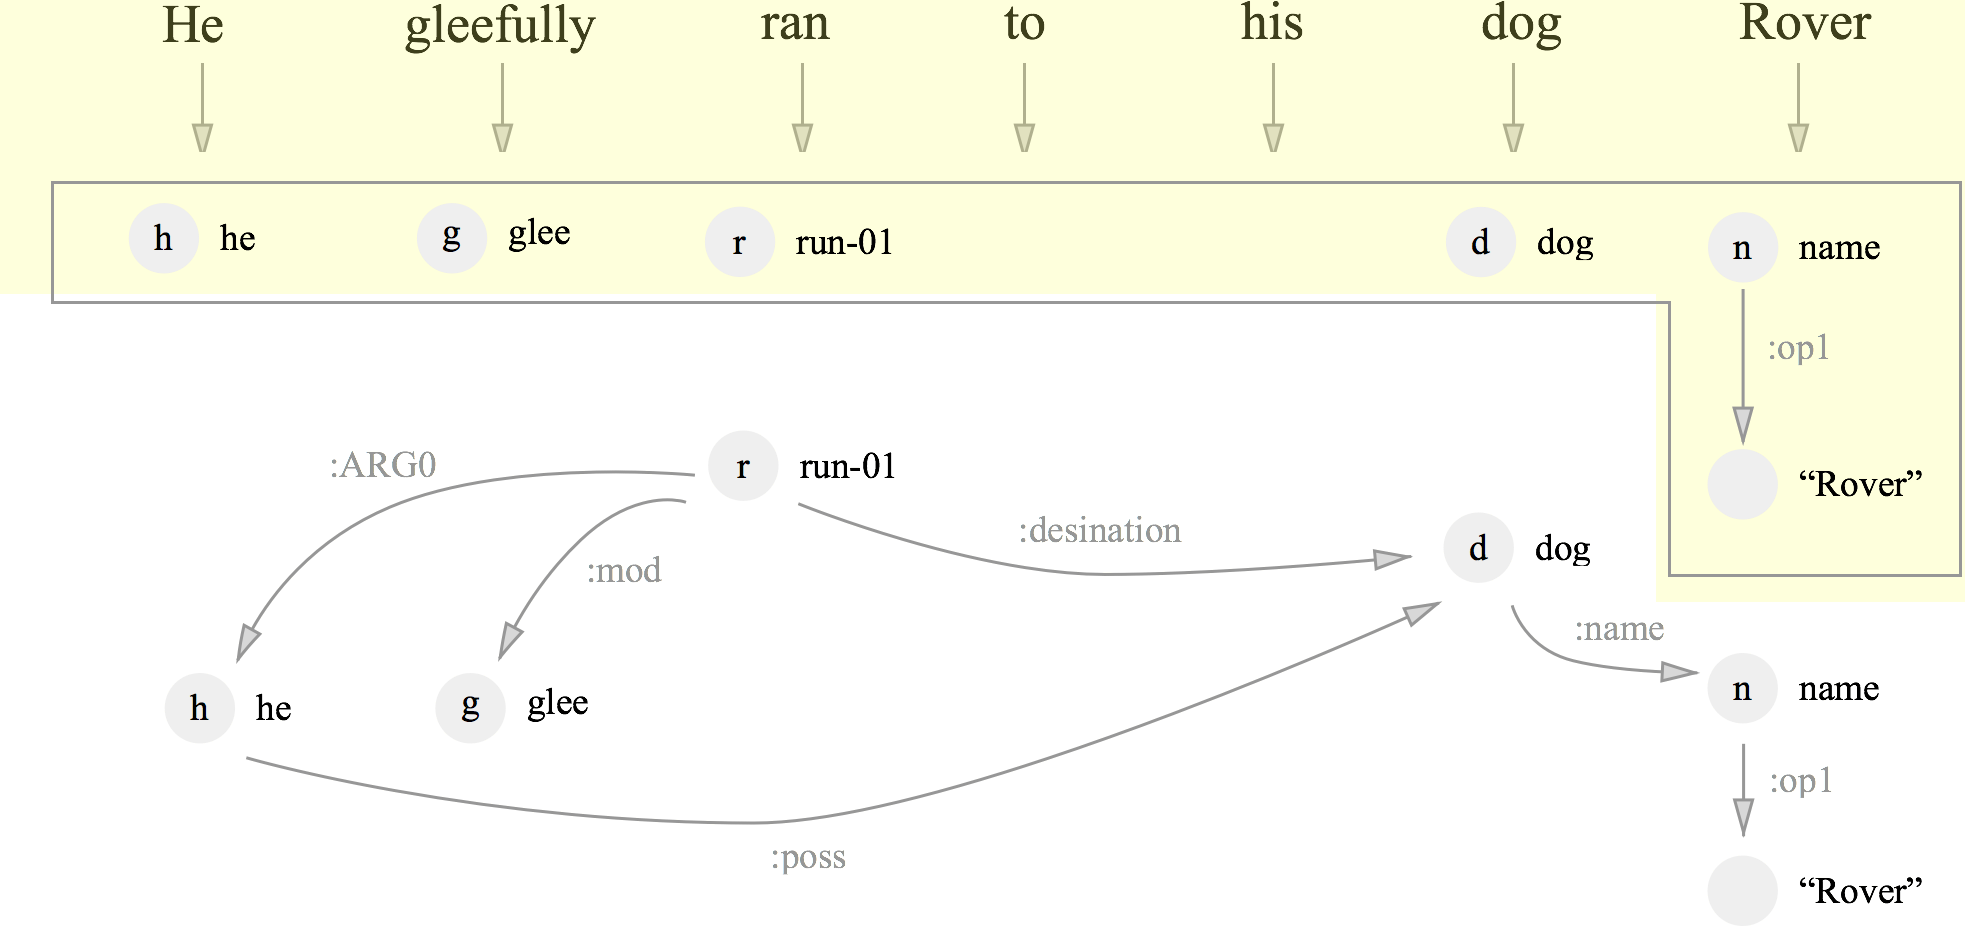
\includegraphics[scale=0.17]{concept_hard.png}
\end{center}
\end{frame}

\begin{frame}[noframenumbering]{Observation: NER++ is Surprisingly Hard}
\hh{From Flanigan et al. (2014):}

\begin{center}
\begin{tabular}{lccc}
\hline
System & Precision & Recall & F$_1$ \\
\hline
Gold NER++      & 76 & 84 & 80 \\
Predicted NER++ & 52 & 66 & 58 \\
\hline
\end{tabular}
\end{center}

\begin{itemize}
\item 22\% Performance loss on NER++
\item Even larger than the 20\% performance loss on SRL++
\end{itemize}
\end{frame}

%%%%%%%%%%%%%%%%%%% 
% Contribution: Actions
%%%%%%%%%%%%%%%%%%%
\begin{frame}{Contribution: Factor NER++ into \textit{Actions}}
\begin{center}
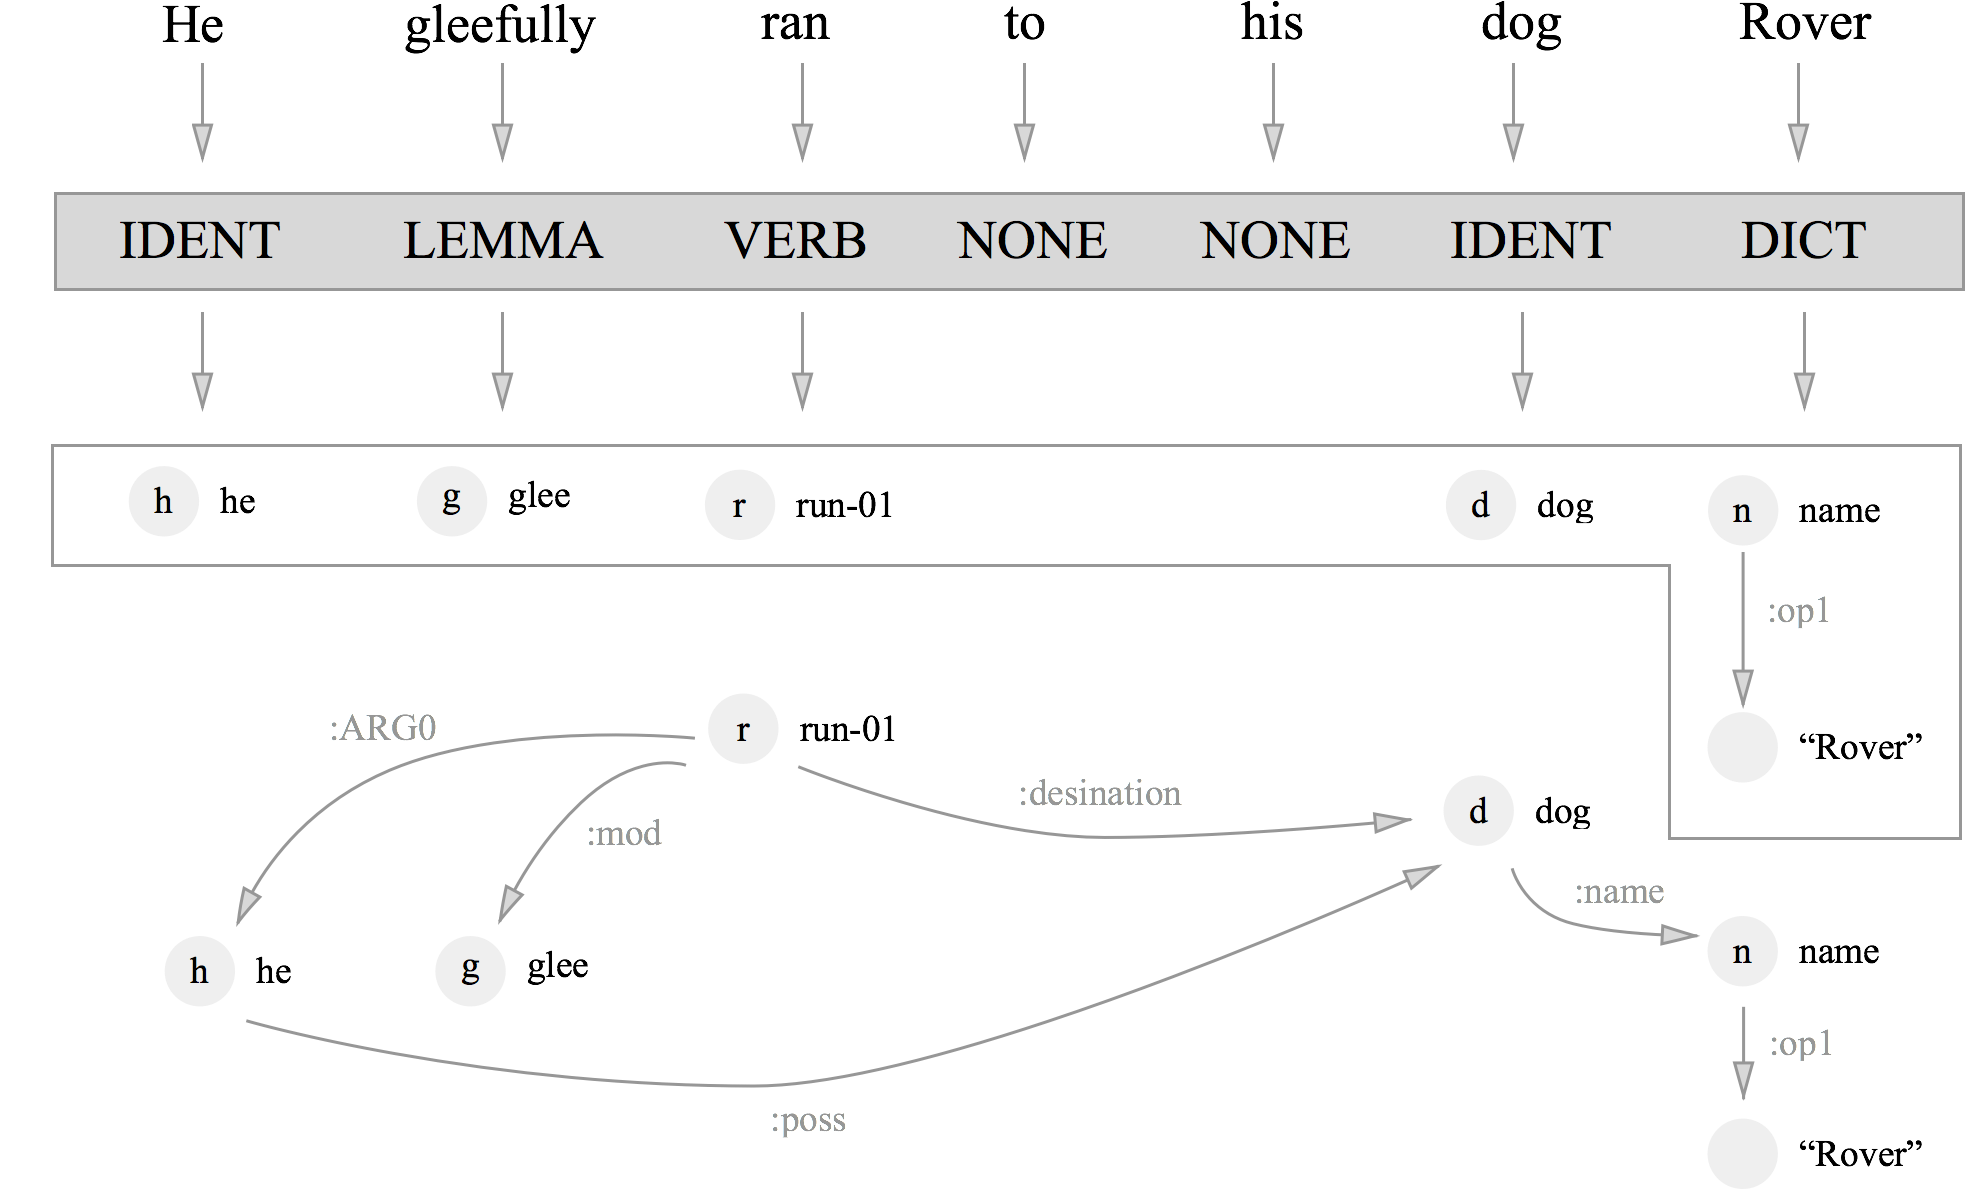
\includegraphics[scale=0.17]{concept.png}
\end{center}
\end{frame}

%%%%%%%%%%%%%%%%%%% 
% List Actions
%%%%%%%%%%%%%%%%%%%
\begin{frame}{Contribution: Factor NER++ into \textit{Actions}}
\hh{9 actions:}
\begin{center}
\begin{tabular}{ll}
\hh{Identity}  & Generate node with token's name. \\
\hh{Lemma}     & Generate node with token's lemma. \\
\hh{Verb}      & Generate node from a token's verb sense. \\
\\
\pause
\hh{Name}      & Generate an NER node (e.g., \w{dog Fido}). \\
\hh{Person}    & A special case of \textbf{Name} for people. \\
\\
\pause
\hh{Date}      & Convert Timex to AMR date node. \\
\hh{Value}     & Parse a textual number. \\
\\
\pause
\hh{None}      & Generate nothing. \\
\\
\pause
\hh{Dict}      & Lookup this word in a mapping. \\
\end{tabular}
\end{center}
\end{frame}

%%%%%%%%%%%%%%%%%%% 
% Dict
%%%%%%%%%%%%%%%%%%%
\begin{frame}{The Dict Action}
\begin{itemize}

\item A ``catch-all'' for nodes that aren't common actions.

\begin{center}
\begin{tabular}{lcl}
\w{``Sailor''} &
$\rightarrow$ &
\raisebox{-.5\height}{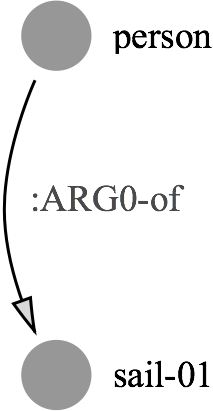
\includegraphics[scale=0.20]{sailor.png}}
\end{tabular}
\end{center}
\pause

\item Only 26\% of tokens.

\item How do we learn this mapping?
\pause
\begin{itemize}
  \item Now that you mention it, how do we learn any of the actions?
  \pause
  \item Induce an \textit{alignment} from nodes to tokens.
  \pause
  \item (Dict action just takes the most common alignment).
  \item (Actions train from the induced alignments).
\end{itemize}
\end{itemize}
\end{frame}

%%%%%%%%%%%%%%%%%%% 
% Alignments
%%%%%%%%%%%%%%%%%%%
\begin{frame}{Alignments}
\begin{itemize}
\item For each node in the AMR, pick a single token it aligns to.
\item Prior work: rule-based alignment or IBM model.
\pause
\vspace{2em}
\item We have one more factor to consider...
\end{itemize}
\end{frame}

%%%%%%%%%%%%%%%%%%% 
% Action Reliability
%%%%%%%%%%%%%%%%%%%
\begin{frame}{Aside: Action Reliability}
\hh{How likely are we to get the right node if we got the right action?} \\
\pause
\vspace{2em}
\hh{Not all actions are equally reliable:}
\begin{center}
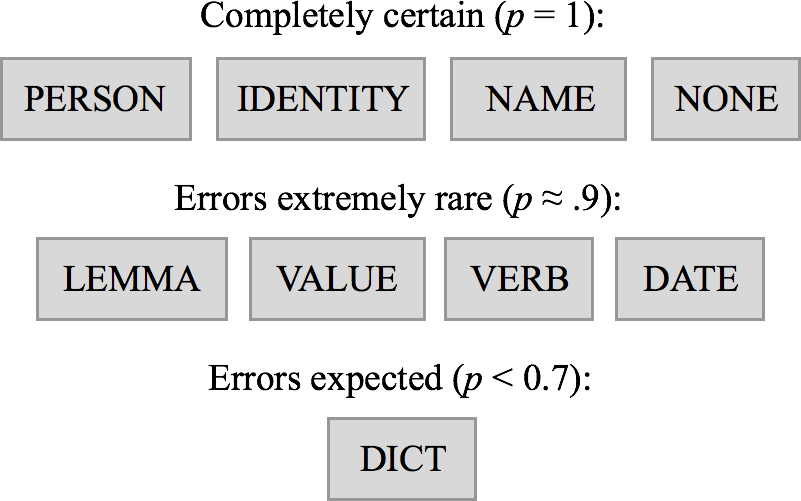
\includegraphics[scale=0.20]{informativeness.png}
\end{center}
\end{frame}

%%%%%%%%%%%%%%%%%%% 
% Alignments
%%%%%%%%%%%%%%%%%%%
\begin{frame}{Alignments}
\begin{itemize}
\item For each node in the AMR, pick a single token it aligns to.
\item Prior work: rule-based alignment or IBM model.
\vspace{2em}
\item We also want alignments that generate reliable actions.
\pause
\vspace{2em}
\item Formulate as a Boolean LP optimizing for reliable actions.
\item Yields $\sim$ 1 F$_1$ improvement on end-to-end parsing.
\end{itemize}
\end{frame}


%%%%%%%%%%%%%%%%%%% 
% Results
%%%%%%%%%%%%%%%%%%%
\begin{frame}{Results}
\begin{itemize}
  \item Incorporate our NER++ into JAMR SRL++:
\end{itemize}

\begin{center}
\begin{tabular}{l|l|llr}
\textbf{Dataset} &  \textbf{System} & \textbf{P} & \textbf{R} & \textbf{F$_1$} \\
\hline
\multirow{2}{*}{2014T12} & JAMR & \textbf{67.1} & 53.2 & 59.3 \\
  & \textbf{Our System} & 66.6 & \textbf{58.3} & \textbf{62.2} \\
\hline
\multirow{2}{*}{2013E117} & JAMR & \textbf{66.9} & 52.9 & 59.1 \\
  & \textbf{Our System} & 65.9 & \textbf{59.0} & \textbf{62.3} \\
\end{tabular}
\end{center}

\begin{itemize}
  \item 3 F$_1$ improvement.
  \item Minimum 5 point improvement in recall.
\end{itemize}
\end{frame}

%%%%%%%%%%%%%%%%%%% 
% THANKS
%%%%%%%%%%%%%%%%%%%
\begin{frame}{Thanks!}
\begin{center}
\hh{Questions?} \\
\vspace{1em}
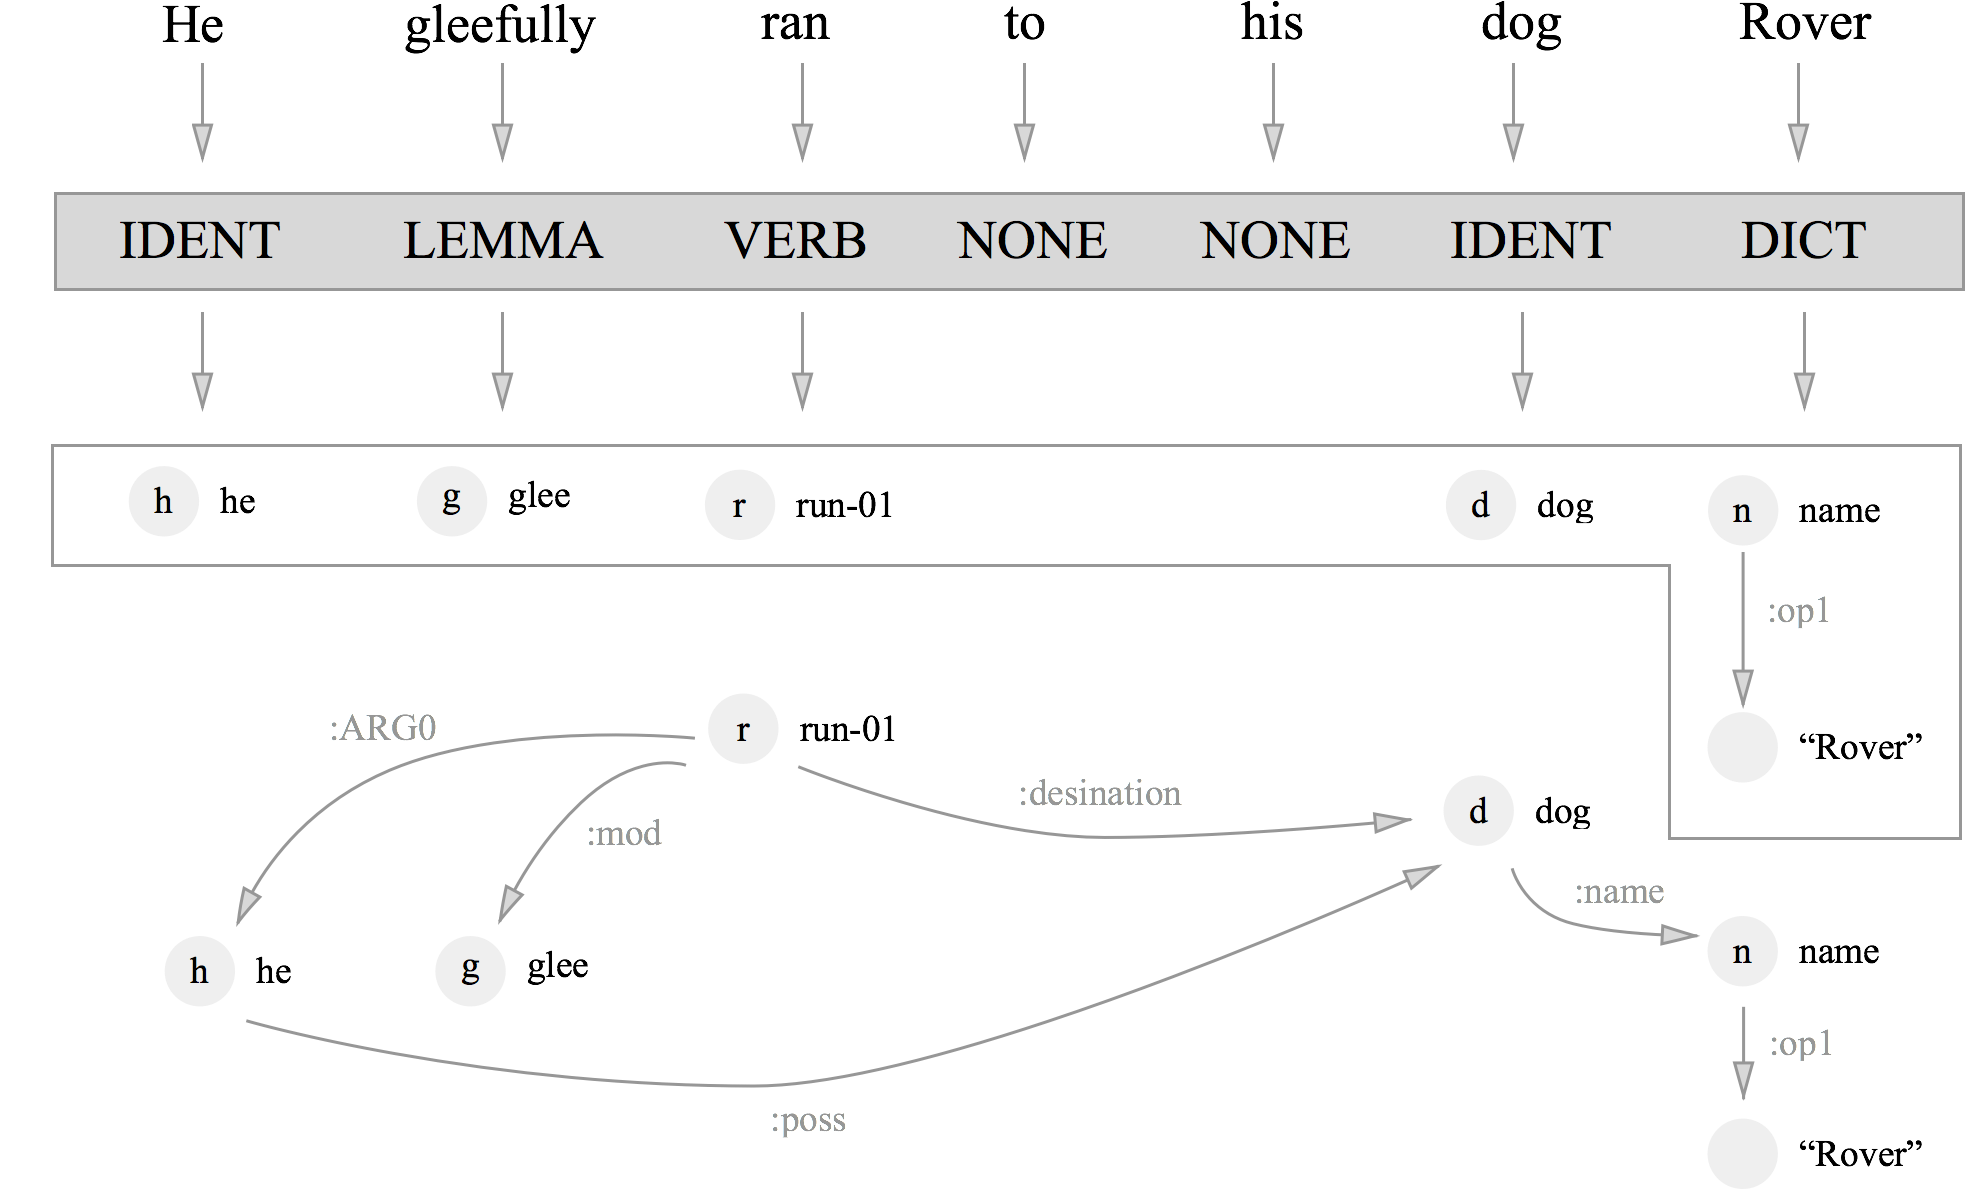
\includegraphics[scale=0.15]{concept.png}
\end{center}
\end{frame}


\end{document}
